\documentclass[12pt, a4paper]{article}

% ============================================================
% PACOTES
% ============================================================
\usepackage[utf8]{inputenc}
\usepackage[T1]{fontenc}
\usepackage[brazil]{babel}
\usepackage{geometry}
\usepackage{listings}
\usepackage{xcolor}
\usepackage{fancyhdr}
\usepackage{amsmath}
\usepackage{amssymb}
\usepackage{indentfirst}
\usepackage{setspace}
\usepackage{booktabs}
\usepackage[pdftex]{graphicx}
\usepackage{caption}
\usepackage{hyperref}
\usepackage{colortbl}
\usepackage{textcomp}
\usepackage[pdftex]{color}
\usepackage{array}
\usepackage{titlesec}
\usepackage{mdframed}

% ============================================================
% CORES
% ============================================================
\definecolor{azulescuro}{RGB}{27,42,74}
\definecolor{azulmedio}{RGB}{74,111,165}
\definecolor{cinzaclaro}{RGB}{242,242,242}
\definecolor{verdesuave}{RGB}{217,234,211}

% ============================================================
% ESTILO DAS SECOES
% ============================================================
\titleformat{\section}[block]
  {\normalfont\large\bfseries\color{azulescuro}}
  {}{0em}{}[\color{azulescuro}\titlerule]
\titlespacing*{\section}{0pt}{12pt}{6pt}

\titleformat{\subsection}[block]
  {\normalfont\normalsize\bfseries\color{azulmedio}}
  {}{0em}{}
\titlespacing*{\subsection}{0pt}{10pt}{4pt}

% ============================================================
% ESTILO DAS TABELAS
% ============================================================
\newcommand{\headerrow}{\rowcolor{azulescuro}}
\newcommand{\altrow}{\rowcolor{cinzaclaro}}

% Redefine toprule/midrule/bottomrule com cor azul
\setlength{\arrayrulewidth}{0.5pt}
\arrayrulecolor{azulescuro}

% ============================================================
% CONFIGURACOES DE PAGINA - Formato SBC
% ============================================================
\geometry{top=3cm, bottom=2.5cm, left=3cm, right=2cm}
\setlength{\headheight}{14pt}
\addtolength{\topmargin}{-2pt}

% ============================================================
% CABECALHO ELEGANTE
% ============================================================
\pagestyle{fancy}
\fancyhf{}
\fancyhead[L]{\small\textcolor{azulescuro}{\textbf{Claudineia Moreira de Oliveira}}}
\fancyhead[R]{\small\textcolor{azulescuro}{Análise de Custos -- Galpão Logístico}}
\fancyfoot[C]{\textcolor{azulescuro}{\small\thepage}}
\renewcommand{\headrulewidth}{1.5pt}
\renewcommand{\headrule}{\hbox to\headwidth{\color{azulescuro}\leaders\hrule height \headrulewidth\hfill}}
\renewcommand{\footrulewidth}{0.4pt}
\renewcommand{\footrule}{\hbox to\headwidth{\color{azulescuro}\leaders\hrule height \footrulewidth\hfill}}

% ============================================================
% CONFIGURACAO DO CODIGO C++
% ============================================================
\lstset{
    language=C++,
    basicstyle=\ttfamily\small,
    keywordstyle=\color{blue}\bfseries,
    commentstyle=\color{gray}\itshape,
    stringstyle=\color{red},
    numberstyle=\tiny\color{gray},
    numbers=left,
    stepnumber=1,
    breaklines=true,
    frame=single,
    frameround=tttt,
    backgroundcolor=\color{gray!10},
    showstringspaces=false,
    tabsize=4,
    literate=
        {á}{{\'a}}1 {é}{{\'e}}1 {í}{{\'i}}1 {ó}{{\'o}}1 {ú}{{\'u}}1
        {â}{{\^a}}1 {ê}{{\^e}}1 {ô}{{\^o}}1 {ã}{{\~a}}1 {õ}{{\~o}}1
        {ç}{{\c{c}}}1 {Á}{{\'A}}1 {É}{{\'E}}1 {Ã}{{\~A}}1
}

% ============================================================
% DOCUMENTO
% ============================================================
\begin{document}

% ---- TITULO ----
\begin{center}
    \colorbox{azulescuro}{\parbox{\textwidth}{\centering\vspace{0.3cm}
    {\large \textcolor{white}{\textbf{UNIVERSIDADE FEDERAL FLUMINENSE -- UFF -- Volta Redonda}}} \\[0.2cm]
    {\normalsize \textcolor{white}{Programa de Pós-Graduação em Modelagem Computacional}} \\[0.1cm]
    {\normalsize \textcolor{white}{Disciplina: Estrutura de Dados e Algoritmos \quad | \quad Professor: Thiago Neves}}
    \vspace{0.3cm}}} \\[0.4cm]
    {\LARGE \textbf{\textcolor{azulescuro}{Análise de Custos para Instalação de Galpão Logístico\\
    Utilizando Grafos e Algoritmos de Caminho Mínimo}}} \\[0.3cm]
    \textcolor{azulescuro}{\rule{\linewidth}{1.5pt}} \\[0.2cm]
    {\normalsize \textbf{Claudineia Moreira de Oliveira}} \\[0.1cm]
    {\normalsize \textit{Junho de 2026}}
\end{center}

\vspace{0.3cm}

% ---- ABSTRACT ----
\noindent\textit{\textbf{Abstract.} This paper presents a computational system for decision support in the installation of logistics warehouses in 15 real neighborhoods of Extrema, Minas Gerais. The problem is modeled as an undirected weighted graph. Three shortest path algorithms are implemented and compared: Dijkstra, Bellman-Ford and Floyd-Warshall, with statistical analysis over 30 repetitions per origin vertex. The system determines the neighborhood with the lowest total deployment cost defined by \textit{custoGalp\~ao = custoInstala\c{c}\~ao $-$ custoOpera\c{c}\~aoAnual}. The implementation uses Object-Oriented Programming in C++ with a Graph ADT, with Big-O complexity analysis.}

\vspace{0.2cm}
\noindent\textit{\textbf{Keywords.} graphs; shortest path; Dijkstra; Bellman-Ford; Floyd-Warshall; logistics; ADT; object-oriented programming.}

\vspace{0.3cm}

% ---- RESUMO ----
\noindent\textbf{Resumo.} Este trabalho apresenta um sistema computacional para apoio à decisão na instalação de galpões logísticos em 15 bairros reais de Extrema, Minas Gerais. O problema é modelado como um grafo \textit{não direcionado} ponderado. Três algoritmos de caminho mínimo são implementados e comparados: \textit{Dijkstra}, \textit{Bellman-Ford} e \textit{Floyd-Warshall}, com análise estatística sobre 30 repetições por vértice de origem. O sistema determina o bairro de menor \textit{custoGalp\~ao = custoInstala\c{c}\~ao $-$ custoOpera\c{c}\~aoAnual}. A implementação utiliza Orientação a Objetos em C++ com TAD Grafo e análise de complexidade Big-O.

\vspace{0.2cm}
\noindent\textbf{Palavras-chave.} grafos; caminho mínimo; Dijkstra; Bellman-Ford; Floyd-Warshall; logística; TAD; orientação a objetos.

\vspace{0.4cm}

% ============================================================
% 1. INTRODUCAO
% ============================================================
\section*{1. INTRODUÇÃO}

A escolha da localização de galpões logísticos constitui uma decisão estratégica de alto impacto financeiro para empresas do setor. Extrema, localizada no extremo sul de Minas Gerais na divisa com São Paulo, consolidou-se como um dos principais polos logísticos do Brasil, com estoque superior a 650 mil m$^2$ às margens da Rodovia Fernão Dias (BR-381). Seus incentivos fiscais e posição geográfica privilegiada atraíram empresas de grande porte como Mercado Livre e Magazine Luiza \cite{cushman2022, gala2023}.

A escolha de Extrema como objeto de estudo é motivada tanto pela literatura quanto pela experiência profissional da autora. Segundo Gala (2023) \cite{gala2023}, o polo industrial de Extrema tem sua origem na localização estratégica da cidade na divisa entre Minas Gerais e São Paulo. Venceslau e Lima (2024) \cite{venceslau2024}, em artigo publicado na revista \textit{Caminhos de Geografia} (Qualis A1), atribuem a Extrema a primazia na logística de \textit{e-commerce} no Brasil. A Redação E-Commerce Brasil \cite{ecommerce2023} denomina o fenômeno como o paradoxo logístico do Brasil.

No âmbito profissional, a autora atuou como analista de sistemas e gerente de projetos de TI em empresa do setor, visitando pessoalmente Extrema para viabilizar um projeto logístico. Esta experiência, aliada ao crescimento documentado da cidade \cite{cushman2022, gala2023, venceslau2024, ecommerce2023}, confere ao problema proposto relevância acadêmica e motivação concreta.

Este trabalho propõe um sistema computacional baseado em grafos não direcionados ponderados para modelar 15 bairros reais de Extrema e calcular os custos logísticos de instalação para cada candidato. Para o cálculo das distâncias mínimas são implementados e comparados os algoritmos de \textit{Dijkstra} \cite{dijkstra1959}, \textit{Bellman-Ford} \cite{bellman1958} e \textit{Floyd-Warshall} \cite{cormen2009}. A implementação é desenvolvida em C++ com Orientação a Objetos, estruturada em um TAD Grafo.

O restante deste artigo está organizado da seguinte forma: a Seção 2 apresenta o embasamento teórico; a Seção 3 descreve o TAD Grafo; a Seção 4 apresenta a análise de complexidade; a Seção 5 compara os três algoritmos; a Seção 6 descreve o ambiente experimental; a Seção 7 apresenta os resultados; e a Seção 8 conclui o trabalho.

% ============================================================
% 2. EMBASAMENTO TEORICO
% ============================================================
\section*{2. EMBASAMENTO TEÓRICO}

\subsection*{2.1 Grafos Não Direcionados Ponderados}

Um grafo $G = (V, E)$ é composto por um conjunto de vértices $V$ e arestas $E$. Quando as arestas possuem peso numérico sem direção definida, o grafo é denominado \textit{não direcionado ponderado}. Um grafo é \textit{conexo} quando existe caminho entre qualquer par de vértices. Para grafos esparsos, a \textit{lista de adjacência} é a representação mais eficiente em termos de memória \cite{neves2026a, dasgupta2006}.

\subsection*{2.2 Algoritmo de Dijkstra}

O algoritmo de \textit{Dijkstra} \cite{dijkstra1959} resolve o problema do caminho mínimo de única origem (\textit{Single-Source Shortest Path}) em grafos com pesos estritamente positivos. Seja $D[v]$ a distância mínima da origem ao vértice $v$ e $c[u,v]$ o custo da aresta $(u,v)$. O algoritmo inicializa $D[\text{origem}] = 0$ e $D[v] = \infty$ para os demais. A cada iteração, o vértice $w$ com menor $D[w]$ é selecionado e as estimativas são atualizadas: $D[v] = \min(D[v], D[w] + c[w,v])$. Na implementação por array simples, a complexidade é $O(n^2)$ \cite{cormen2009, sedgewick2011}.

\subsection*{2.3 Algoritmo de Bellman-Ford}

O algoritmo de \textit{Bellman-Ford} \cite{bellman1958} resolve o caminho mínimo para o caso geral, suportando arestas de peso negativo. Realiza $|V|-1$ iterações de relaxamento sobre todas as arestas: se $D[u] + c[u,v] < D[v]$, então $D[v]$ é atualizado. Detecta ciclos negativos na $n$-ésima iteração. Sua complexidade é $O(n \times a)$ \cite{bellman1958, cormen2009}.

\subsection*{2.4 Algoritmo de Floyd-Warshall}

O algoritmo de \textit{Floyd-Warshall} \cite{cormen2009} resolve o problema do caminho mínimo entre todos os pares de vértices (\textit{All-Pairs Shortest Path}). Para cada vértice intermediário $k$, verifica se $\text{dist}[i][k] + \text{dist}[k][j] < \text{dist}[i][j]$, atualizando a menor distância entre $i$ e $j$. Sua complexidade é $O(n^3)$ pois utiliza três laços aninhados sobre os $n$ vértices. Admite arestas de peso negativo sem ciclos negativos. Neste trabalho, extrai-se apenas a linha da origem, produzindo resultado equivalente ao \textit{Dijkstra} e \textit{Bellman-Ford} \cite{cormen2009, dasgupta2006}.

\subsection*{2.5 Notação Assintótica Big-O}

A notação \textit{Big-O} \cite{neves2026a} expressa o comportamento assintótico de pior caso: $g(n)$ é $O(f(n))$ se existem constantes $c > 0$ e $k > 0$ tais que $g(n) \leq c \times f(n)$ para todo $n \geq k$.

\subsection*{2.6 Tipo Abstrato de Dado (TAD)}

Um TAD é definido exclusivamente por sua interface de operações, sem expor detalhes de implementação \cite{neves2026a}. A Orientação a Objetos em C++ implementa este conceito com classes com modificadores \textit{public} e \textit{private}, construtores, destrutores e métodos de acesso \cite{neves2026b}.

% ============================================================
% 3. IMPLEMENTACAO DO TAD GRAFO
% ============================================================
\section*{3. IMPLEMENTAÇÃO DO TAD GRAFO}

\subsection*{3.1 Estrutura de Classes}

O TAD Grafo foi implementado em C++ com quatro classes com encapsulamento completo. A Tabela 1 descreve cada classe.

\begin{table}[h!]
\centering
\caption{Classes do TAD Grafo}
\begin{tabular}{>{\bfseries\itshape}lp{9cm}}
\rowcolor{azulescuro}
\textcolor{white}{\textbf{Classe}} & \textcolor{white}{\textbf{Responsabilidade}} \\
\textit{Vertice} & Bairro candidato: id, custo de instalação e 12 demandas mensais \\
\textit{Aresta}  & Conexão entre bairros: origem, destino e custo de transporte \\
\textit{No}      & Elemento da lista de adjacência: ponteiro para Aresta e próximo No \\
\textit{Grafo}   & TAD principal: lista de adjacência, Dijkstra, Bellman-Ford, Floyd-Warshall \\
\bottomrule
\end{tabular}
\label{tab:classes}
\end{table}
\vspace{-0.3cm}
\begin{center}\small\textit{Fonte: Os autores (2026).}\end{center}

\subsection*{3.2 Interface Pública do TAD}

Os métodos públicos da classe \textit{Grafo} constituem a interface do TAD:

\begin{lstlisting}
Grafo(int numVertices, int numArestas)   ~Grafo()
void addVertice(int id, double custo, int* demanda)
void addAresta(int origem, int destino, double custo)
Vertice* getVertice(int id)   bool isEmpty()
int getNumVertices()          int getNumArestas()
void dijkstra(int origem, double* distancias)
void bellmanFord(int origem, double* distancias)
void floydWarshall(int origem, double* distancias)
double custoOperacaoMensal(int orig, int mes, double* dist)
double custoOperacaoAnual(int orig)
int melhorBairro()
\end{lstlisting}

A representação interna utiliza lista de adjacência não direcionada. O método \textit{addAresta} insere a aresta nos dois sentidos (origem$\rightarrow$destino e destino$\rightarrow$origem), garantindo o comportamento não direcionado sem alterar os arquivos de entrada \cite{neves2026a, dasgupta2006}.

% ============================================================
% 4. ANALISE DE COMPLEXIDADE
% ============================================================
\section*{4. ANÁLISE DE COMPLEXIDADE}

A Tabela 2 apresenta a análise de complexidade assintótica dos métodos do TAD, onde $n = |V|$ é o número de vértices e $a = |E|$ é o número de arestas.

\begin{table}[h!]
\centering
\caption{Complexidade assintótica dos métodos do TAD Grafo}
\small
\begin{tabular}{lll}
\toprule
\textbf{Método} & \textbf{Complexidade} & \textbf{Justificativa} \\
\midrule
Construtor / Destrutor & $O(n)$ / $O(n+a)$ & Inicializa $n$ posições / percorre vértices e arestas \\
isEmpty() / getNumVertices() / getNumArestas() & $O(1)$ & Retorno direto de atributo \\
indiceVertice() / getVertice() / addVertice() & $O(n)$ & Busca linear no array de vértices \\
addAresta() & $O(n)$ & indiceVertice() $O(n)$ + 2 inserções $O(1)$ \\
menorDistancia() & $O(n)$ & Busca linear no array de distâncias \\
dijkstra() & $O(n^2)$ & $n$ iterações $\times$ menorDistancia() $O(n)$ \\
bellmanFord() & $O(n \times a)$ & $n-1$ relaxamentos $\times$ percorre $a$ arestas \\
floydWarshall() & $O(n^3)$ & 3 laços aninhados sobre $n$ vértices \\
custoOperacaoMensal() & $O(n)$ & Percorre os $n$ vértices \\
custoOperacaoAnual() & $O(n^2)$ & dijkstra() $O(n^2)$ + 12 $\times$ $O(n)$ \\
melhorBairro() / imprimirCustos() & $O(n^3)$ & $n \times$ custoOperacaoAnual() $O(n^2)$ \\
imprimirGrafo() & $O(n+a)$ & Percorre vértices e arestas \\
\bottomrule
\end{tabular}
\label{tab:complexidade}
\end{table}
\vspace{-0.3cm}
\begin{center}\small\textit{Fonte: Os autores (2026).}\end{center}

O método \textit{melhorBairro()} apresenta a maior complexidade $O(n^3)$, executando \textit{custoOperacaoAnual()} -- de custo $O(n^2)$ -- para cada um dos $n$ vértices. Este comportamento é aceitável para instâncias com número reduzido de bairros candidatos \cite{ballou2006}.

% ============================================================
% 5. COMPARACAO DOS TRES ALGORITMOS
% ============================================================
\section*{5. COMPARAÇÃO ENTRE DIJKSTRA, BELLMAN-FORD E FLOYD-WARSHALL}

Os três algoritmos produzem resultados idênticos para grafos com pesos estritamente positivos. Os tempos de execução foram medidos em \textbf{30 repetições} por vértice de origem, calculando-se média e desvio padrão. A Tabela 3 sintetiza a comparação e a Tabela 4 apresenta os resultados estatísticos obtidos com 15 vértices.

\begin{table}[h!]
\centering
\caption{Comparação entre Dijkstra, Bellman-Ford e Floyd-Warshall}
\small
\begin{tabular}{llll}
\rowcolor{azulescuro}
\textcolor{white}{\textbf{Característica}} & \textcolor{white}{\textbf{Dijkstra}} & \textcolor{white}{\textbf{Bellman-Ford}} & \textcolor{white}{\textbf{Floyd-Warshall}} \\
Complexidade         & $O(n^2)$     & $O(n \times a)$    & $O(n^3)$ \\
Pesos negativos      & Não          & Sim                & Sim \\
Detecta ciclos neg.  & Não          & Sim                & Não \\
Estratégia           & Gulosa       & Prog. dinâmica     & Prog. dinâmica \\
Escopo               & 1 origem     & 1 origem           & Todos os pares \\
Tempo médio (15 vért.) & 0.000003s  & 0.000027s          & 0.000023s \\
Resultados (teste)   & Idênticos    & Idênticos          & Idênticos \\
Indicado p/ problema & Sim \checkmark & Alternativo      & Alternativo \\
\bottomrule
\end{tabular}
\label{tab:comparacao}
\end{table}
\vspace{-0.3cm}
\begin{center}\small\textit{Fonte: Os autores (2026).}\end{center}

\begin{table}[h!]
\centering
\caption{Análise estatística dos tempos de execução (30 repetições, 15 vértices) -- segundos}
\small
\begin{tabular}{lllllll}
\rowcolor{azulescuro}
\textcolor{white}{\textbf{Orig.}} & \textcolor{white}{\textbf{Méd. Dij.}} & \textcolor{white}{\textbf{DP Dij.}} & \textcolor{white}{\textbf{Méd. Bel.}} & \textcolor{white}{\textbf{DP Bel.}} & \textcolor{white}{\textbf{Méd. FW}} & \textcolor{white}{\textbf{DP FW}} \\
1  & 0.000004 & 0.000000 & 0.000033 & 0.000000 & 0.000034 & 0.000000 \\
2  & 0.000003 & 0.000000 & 0.000029 & 0.000000 & 0.000023 & 0.000000 \\
3  & 0.000003 & 0.000000 & 0.000027 & 0.000000 & 0.000023 & 0.000000 \\
4  & 0.000003 & 0.000000 & 0.000027 & 0.000000 & 0.000022 & 0.000000 \\
5  & 0.000003 & 0.000000 & 0.000026 & 0.000000 & 0.000023 & 0.000000 \\
6  & 0.000003 & 0.000000 & 0.000027 & 0.000000 & 0.000024 & 0.000000 \\
7  & 0.000003 & 0.000000 & 0.000026 & 0.000000 & 0.000023 & 0.000000 \\
8  & 0.000003 & 0.000000 & 0.000028 & 0.000000 & 0.000025 & 0.000000 \\
9  & 0.000003 & 0.000000 & 0.000025 & 0.000000 & 0.000025 & 0.000000 \\
10 & 0.000003 & 0.000000 & 0.000025 & 0.000000 & 0.000023 & 0.000000 \\
11 & 0.000003 & 0.000000 & 0.000026 & 0.000000 & 0.000023 & 0.000000 \\
12 & 0.000003 & 0.000000 & 0.000026 & 0.000000 & 0.000022 & 0.000000 \\
13 & 0.000003 & 0.000000 & 0.000025 & 0.000000 & 0.000022 & 0.000000 \\
14 & 0.000003 & 0.000000 & 0.000024 & 0.000000 & 0.000022 & 0.000000 \\
15 & 0.000003 & 0.000000 & 0.000024 & 0.000000 & 0.000022 & 0.000000 \\
\midrule
\textbf{Total} & \textbf{0.000044} & -- & \textbf{0.000390} & -- & \textbf{0.000320} & -- \\
\bottomrule
\end{tabular}
\label{tab:estatistica}
\end{table}
\vspace{-0.3cm}
\begin{center}\small\textit{Fonte: Os autores (2026). Méd. = Média; DP = Desvio Padrão. Ambiente: Intel i5-1334U, Ubuntu 24.04.}\end{center}

O \textit{Dijkstra} foi o mais eficiente (0.000003s), seguido pelo \textit{Floyd-Warshall} (0.000023s) e \textit{Bellman-Ford} (0.000027s). Apesar da complexidade $O(n^3)$ do \textit{Floyd-Warshall}, seu tempo foi próximo ao \textit{Bellman-Ford} $O(n \times a)$ pois o número de arestas (22) é pequeno em relação a $n^2$ (225). O desvio padrão nulo confirma alta estabilidade \cite{dijkstra1959, bellman1958, cormen2009}.

% ============================================================
% 6. AMBIENTE EXPERIMENTAL
% ============================================================
\section*{6. AMBIENTE EXPERIMENTAL E DADOS DE TESTE}

\subsection*{6.1 Ambiente de Hardware e Software}

\begin{lstlisting}[language=bash, frame=none, numbers=none, backgroundcolor=\color{white}]
Dispositivo         : DESKTOP-50V4UVQ
Sistema Operacional : Ubuntu 24.04 LTS (Linux) via VirtualBox
Processador         : 13th Gen Intel(R) Core(TM) i5-1334U (1.30 GHz)
Arquitetura         : 64 bits, processador x64
Memoria RAM         : 16,0 GB (utilizavel: 15,7 GB)
Compilador          : g++ 13.3.0 (Ubuntu 13.3.0-6ubuntu2~24.04.1)
Editor              : Gedit
Linguagem           : C++ (padrao ISO C++11)
Bibliotecas         : stdio.h, stdlib.h, time.h
Ferramenta          : Google Maps (estimativa de distancias)
Compilacao          : g++ Vertice.cpp Aresta.cpp No.cpp Grafo.cpp main.cpp -o analise
\end{lstlisting}

A medição de tempo foi realizada com a função \textit{clock()} da biblioteca \textit{time.h}, pela expressão \texttt{((double)(t2-t1))/CLOCKS\_PER\_SEC}.

\subsection*{6.2 Dados de Teste}

Os dados foram elaborados com base na estrutura logística real de Extrema-MG, contemplando \textbf{15 bairros candidatos} e \textbf{22 arestas} em um grafo não direcionado conexo. As distâncias foram obtidas via \textit{Google Maps} (2026). Os custos de instalação foram estimados com base em dados de mercado \cite{cushman2022}. Ressalta-se que as distâncias são estimativas adequadas para fins acadêmicos; em um projeto real recomenda-se análise mais apurada das condições viárias.

\begin{table}[h!]
\centering
\caption{Dados dos 15 bairros candidatos de Extrema-MG}
\small
\begin{tabular}{llll}
\rowcolor{azulescuro}
\textcolor{white}{\textbf{ID}} & \textcolor{white}{\textbf{Bairro}} & \textcolor{white}{\textbf{Custo Inst. (R\$)}} & \textcolor{white}{\textbf{Adjacentes}} \\
1  & Centro                  & 2.500.000,00  & 2, 3, 8, 10, 12 \\
2  & Distrito Industrial     & 8.500.000,00  & 1, 3, 4, 6 \\
3  & Bairro dos Pires (BR-381) & 4.500.000,00 & 1, 2, 5, 7, 9, 14 \\
4  & São Bráz               & 3.200.000,00  & 2, 5, 11 \\
5  & Bairro dos Tenentes    & 2.800.000,00  & 3, 4, 6, 13 \\
6  & Condomínio Logístico   & 12.000.000,00 & 2, 5, 7, 14 \\
7  & Divisa SP/MG           & 3.800.000,00  & 3, 6, 15 \\
8  & Ponte Alta             & 2.200.000,00  & 1, 10 \\
9  & Pessegueiros           & 3.600.000,00  & 3, 14 \\
10 & Ponte Nova             & 2.100.000,00  & 1, 8 \\
11 & Morbidelli             & 2.800.000,00  & 4, 12 \\
12 & Vila Rica              & 2.300.000,00  & 1, 11 \\
13 & Salto de Baixo \textbf{\textbf{\textasteriskcentered}} & 1.800.000,00 & 5, 15 \\
14 & Parque Logístico       & 5.500.000,00  & 3, 6, 9 \\
15 & Morada da Serra        & 2.600.000,00  & 7, 13 \\
\bottomrule
\end{tabular}
\label{tab:vertices}
\end{table}
\vspace{-0.3cm}
\begin{center}\small\textit{Fonte: Os autores (2026). \textbf{\textasteriskcentered} Bairro selecionado.}\end{center}

% ============================================================
% 7. RESULTADOS E DISCUSSAO
% ============================================================
\section*{7. RESULTADOS E DISCUSSÃO}

A Tabela 5 apresenta os resultados. O \textit{custoGalp\~ao} é calculado por:
$$\text{custoGalp\~ao} = \text{custoInstalação} - \text{custoOperaçãoAnual}$$

\begin{table}[h!]
\centering
\caption{Resultados da análise de custos logísticos -- Extrema-MG (15 bairros)}
\small
\begin{tabular}{lllll}
\rowcolor{azulescuro}
\textcolor{white}{\textbf{ID}} & \textcolor{white}{\textbf{Custo Inst. (R\$)}} & \textcolor{white}{\textbf{Custo Op. Anual (R\$)}} & \textcolor{white}{\textbf{CustoGalpão (R\$)}} & \textcolor{white}{\textbf{Rank}} \\
1  & 2.500.000,00  & 424.158,50   & 2.075.841,50   & 5$^\circ$  \\
2  & 8.500.000,00  & 300.671,00   & 8.199.329,00   & 14$^\circ$ \\
3  & 4.500.000,00  & 396.095,40   & 4.103.904,60   & 10$^\circ$ \\
4  & 3.200.000,00  & 319.778,00   & 2.880.222,00   & 7$^\circ$  \\
5  & 2.800.000,00  & 299.278,50   & 2.500.721,50   & 6$^\circ$  \\
6  & 12.000.000,00 & 275.485,50   & 11.724.514,50  & 15$^\circ$ \\
7  & 3.800.000,00  & 350.653,50   & 3.449.346,50   & 9$^\circ$  \\
8  & 2.200.000,00  & 542.988,80   & 1.657.011,20   & 3$^\circ$  \\
9  & 3.600.000,00  & 340.675,50   & 3.259.324,50   & 8$^\circ$  \\
10 & 2.100.000,00  & 530.428,70   & 1.569.571,30   & 2$^\circ$  \\
11 & 2.800.000,00  & 361.759,50   & 2.438.240,50   & 4$^\circ$  \\
12 & 2.300.000,00  & 393.097,00   & 1.906.903,00   & -- \\
\rowcolor{verdesuave}
\textbf{13 \textbf{\textasteriskcentered}} & \textbf{1.800.000,00} & \textbf{584.365,50} & \textbf{1.215.634,50} & \textbf{1$^\circ$} \\
14 & 5.500.000,00  & 306.698,00   & 5.193.302,00   & 13$^\circ$ \\
15 & 2.600.000,00  & 550.421,50   & 2.049.578,50   & -- \\
\bottomrule
\end{tabular}
\label{tab:resultados}
\end{table}
\vspace{-0.3cm}
\begin{center}\small\textit{Fonte: Os autores (2026). \textbf{\textasteriskcentered} Bairro selecionado. Distâncias via Google Maps.}\end{center}

\begin{figure}[h!]
\centering
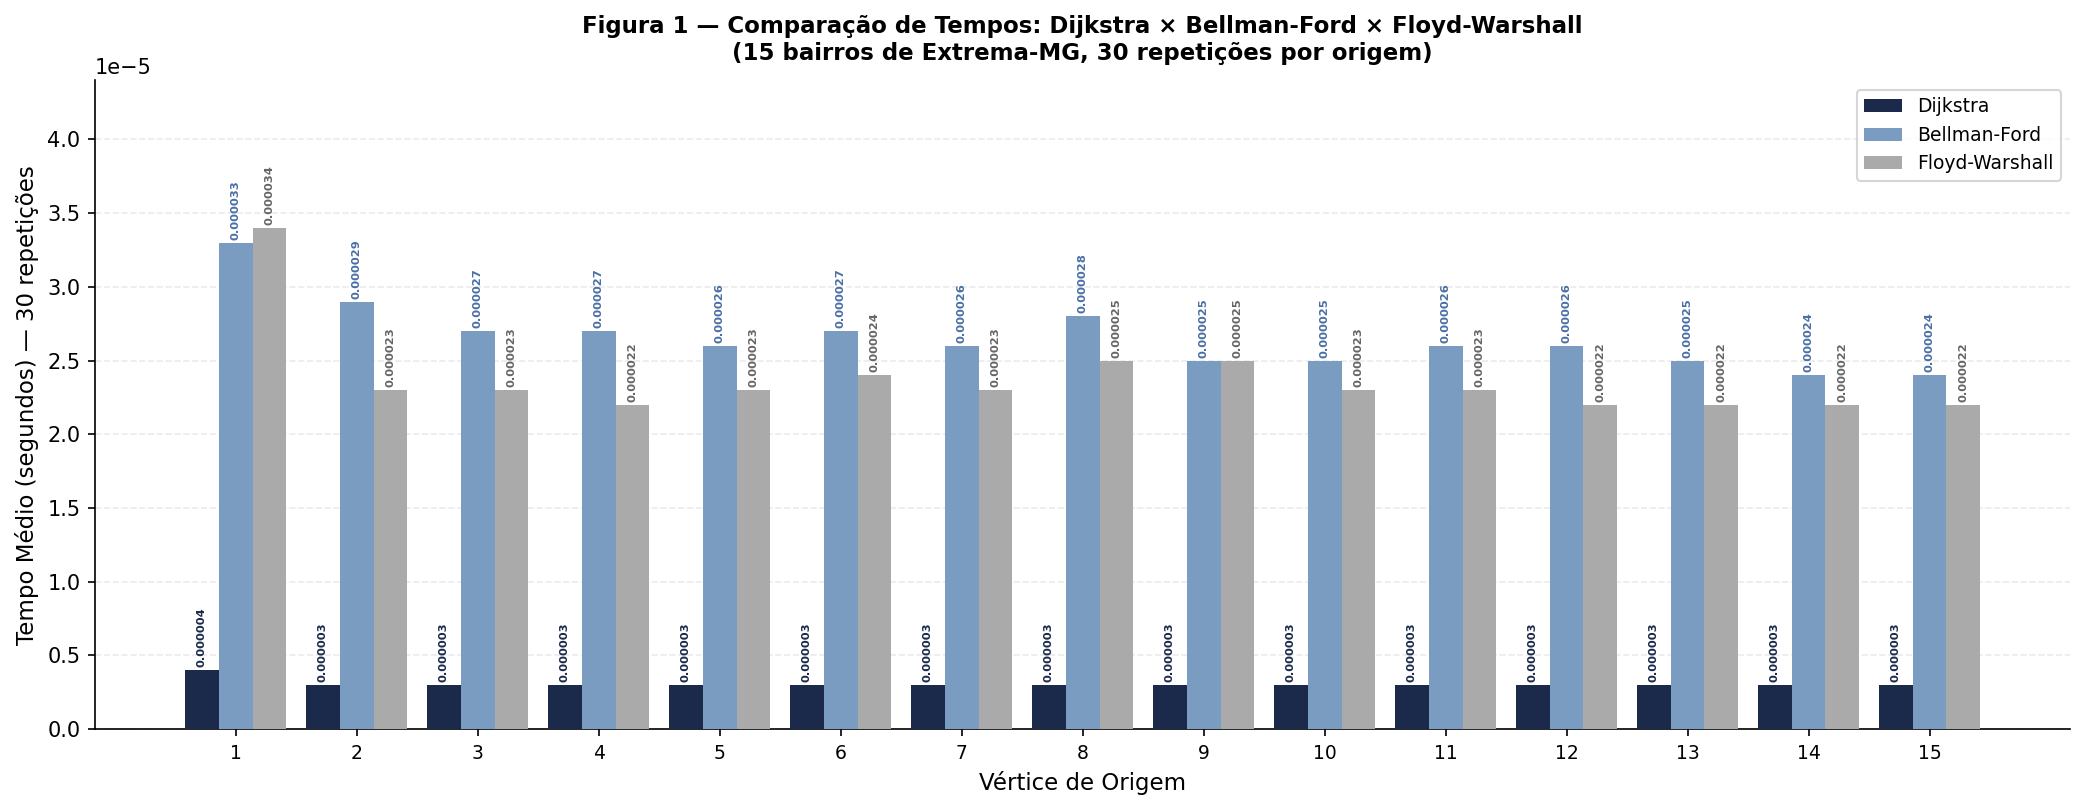
\includegraphics[width=0.95\textwidth, draft=false]{figura1_tempos.png}
\caption{Comparação de tempos de execução: Dijkstra $\times$ Bellman-Ford $\times$ Floyd-Warshall}
\label{fig:tempos}
\end{figure}

\begin{figure}[h!]
\centering
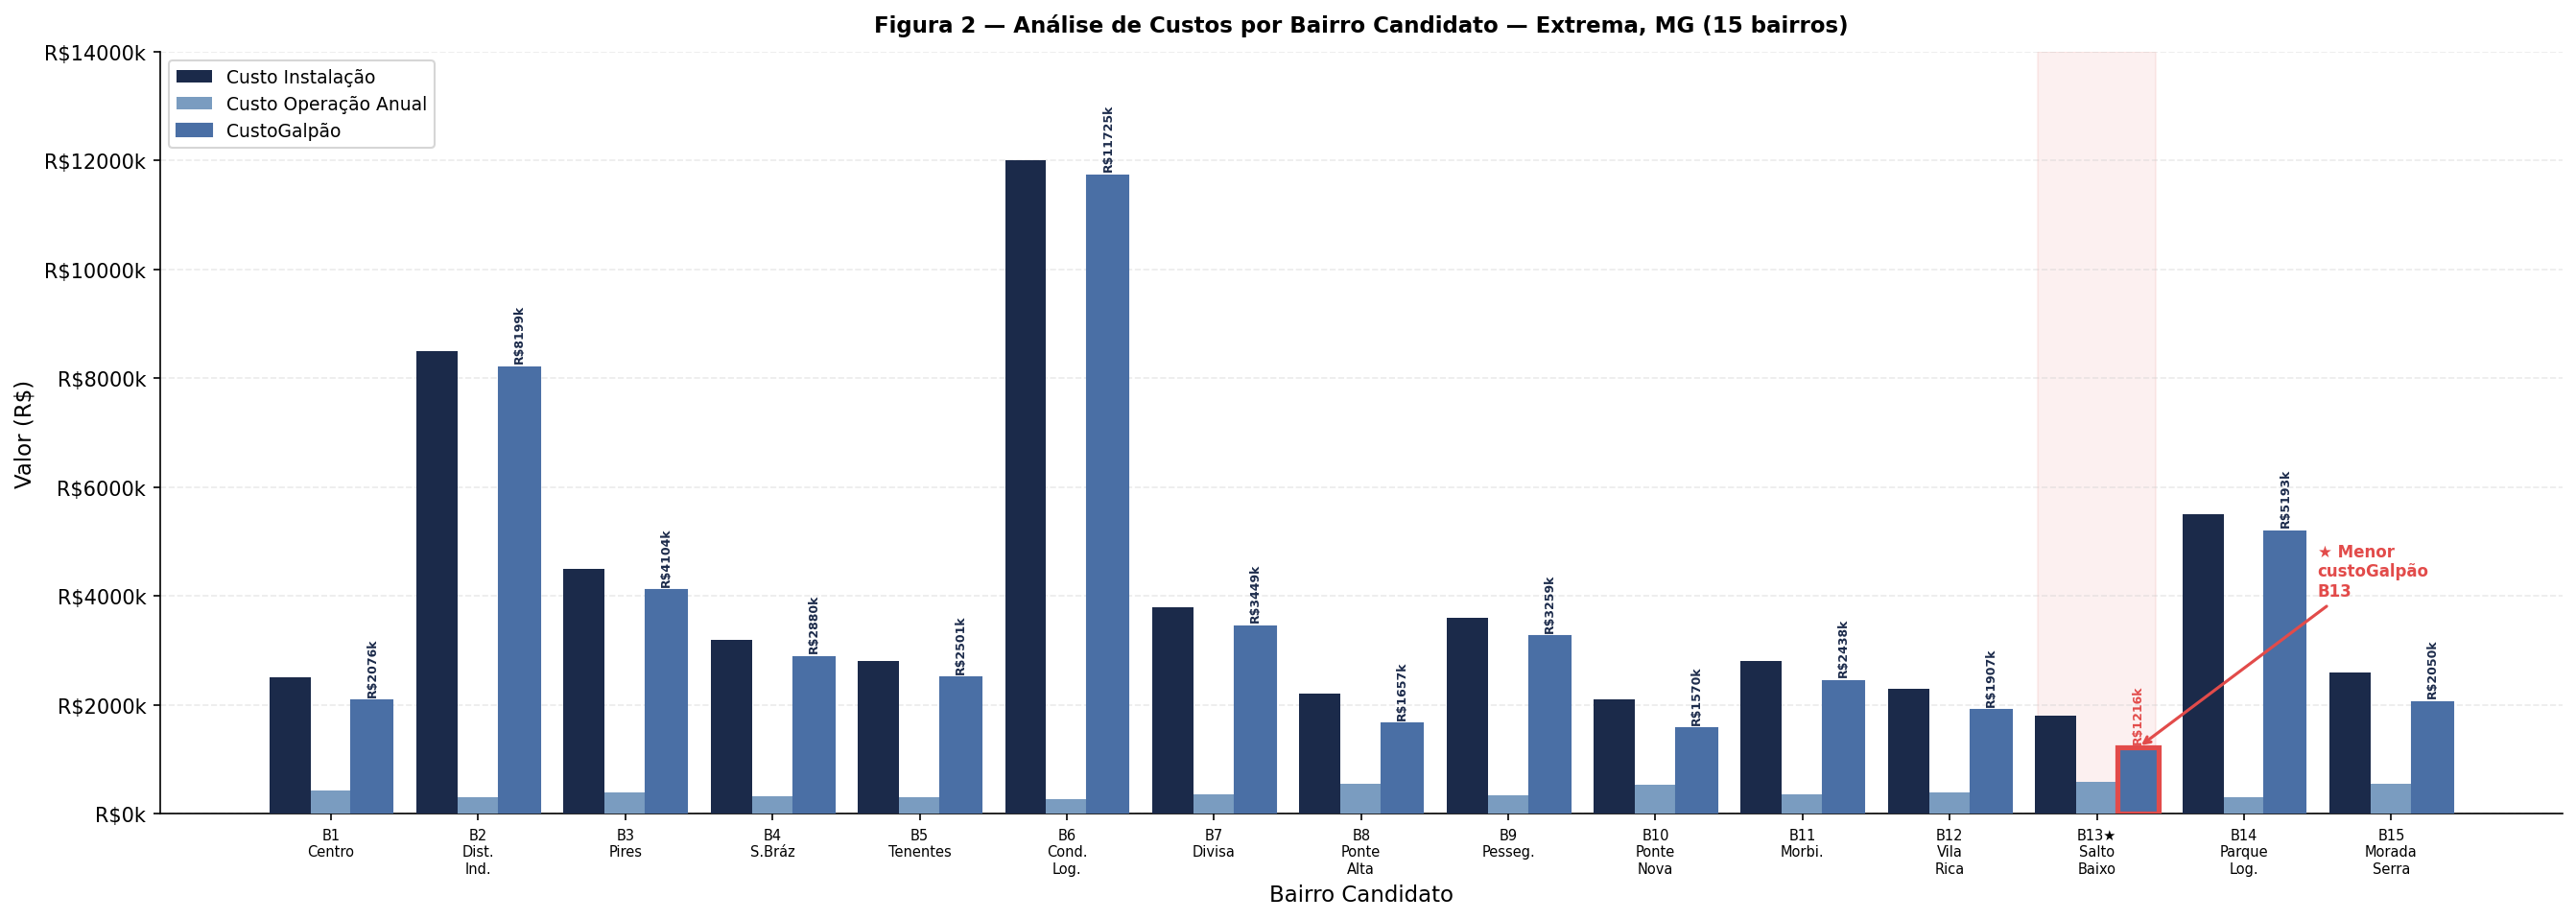
\includegraphics[width=0.95\textwidth]{figura2_custos.png}
\caption{Análise de custos por bairro candidato -- Extrema-MG (R\$)}
\label{fig:custos}
\end{figure}

O Bairro 13 -- Salto de Baixo -- apresentou o menor \textit{custoGalp\~ao} (R\$ 1.215.634,50), sendo indicado como o local mais adequado para instalação do galpão. Este resultado é explicado pelo menor custo fixo de instalação entre todos os candidatos (R\$ 1.800.000,00), que mesmo com custo de operação anual de R\$ 584.365,50, resulta no menor custo total.

O Bairro 6 (Condomínio Logístico) manteve o pior posicionamento (15$^\circ$) com \textit{custoGalp\~ao} de R\$ 11.724.514,50 -- reflexo do elevado custo de instalação de R\$ 12.000.000,00, característico de condomínios Classe A às margens da BR-381. O Bairro 2 (Distrito Industrial) também ficou mal posicionado (14$^\circ$) pelo mesmo motivo.

Quanto ao desempenho dos algoritmos, o \textit{Dijkstra} foi o mais rápido (0.000003s média), seguido pelo \textit{Floyd-Warshall} (0.000023s) e \textit{Bellman-Ford} (0.000027s). Os três produziram resultados idênticos, confirmando a consistência do modelo.

\subsection*{7.1 Análise de Sensibilidade}

Para avaliar a robustez do modelo, realizou-se uma análise de sensibilidade variando os custos de instalação e operação em diferentes percentuais. A Tabela 6 e a Figura 3 apresentam os resultados.

\begin{table}[ht]
\centering
\caption{Análise de sensibilidade — variação dos custos e bairro vencedor}
\small
\begin{tabular}{lllll}
\rowcolor{azulescuro}
\textcolor{white}{\textbf{Cenário}} & \textcolor{white}{\textbf{Var. Inst. (\%)}} & \textcolor{white}{\textbf{Var. Op. (\%)}} & \textcolor{white}{\textbf{Melhor Bairro}} & \textcolor{white}{\textbf{CustoGalpão (R\$)}} \\
Base             & 0\%   & 0\%   & 13 -- Salto de Baixo & 1.215.634,50 \\
Otimista         & -20\% & -20\% & 13 -- Salto de Baixo & 972.507,60   \\
Pessimista       & +20\% & +20\% & 13 -- Salto de Baixo & 1.458.761,40 \\
Alta Instalação  & +50\% & 0\%   & 13 -- Salto de Baixo & 2.115.634,50 \\
Alta Operação    & 0\%   & +50\% & 13 -- Salto de Baixo & 923.451,75   \\
\bottomrule
\end{tabular}
\label{tab:sensibilidade}
\end{table}
\vspace{-0.3cm}
\begin{center}\small\textit{Fonte: Os autores (2026).}\end{center}

\begin{figure}[ht]
\centering
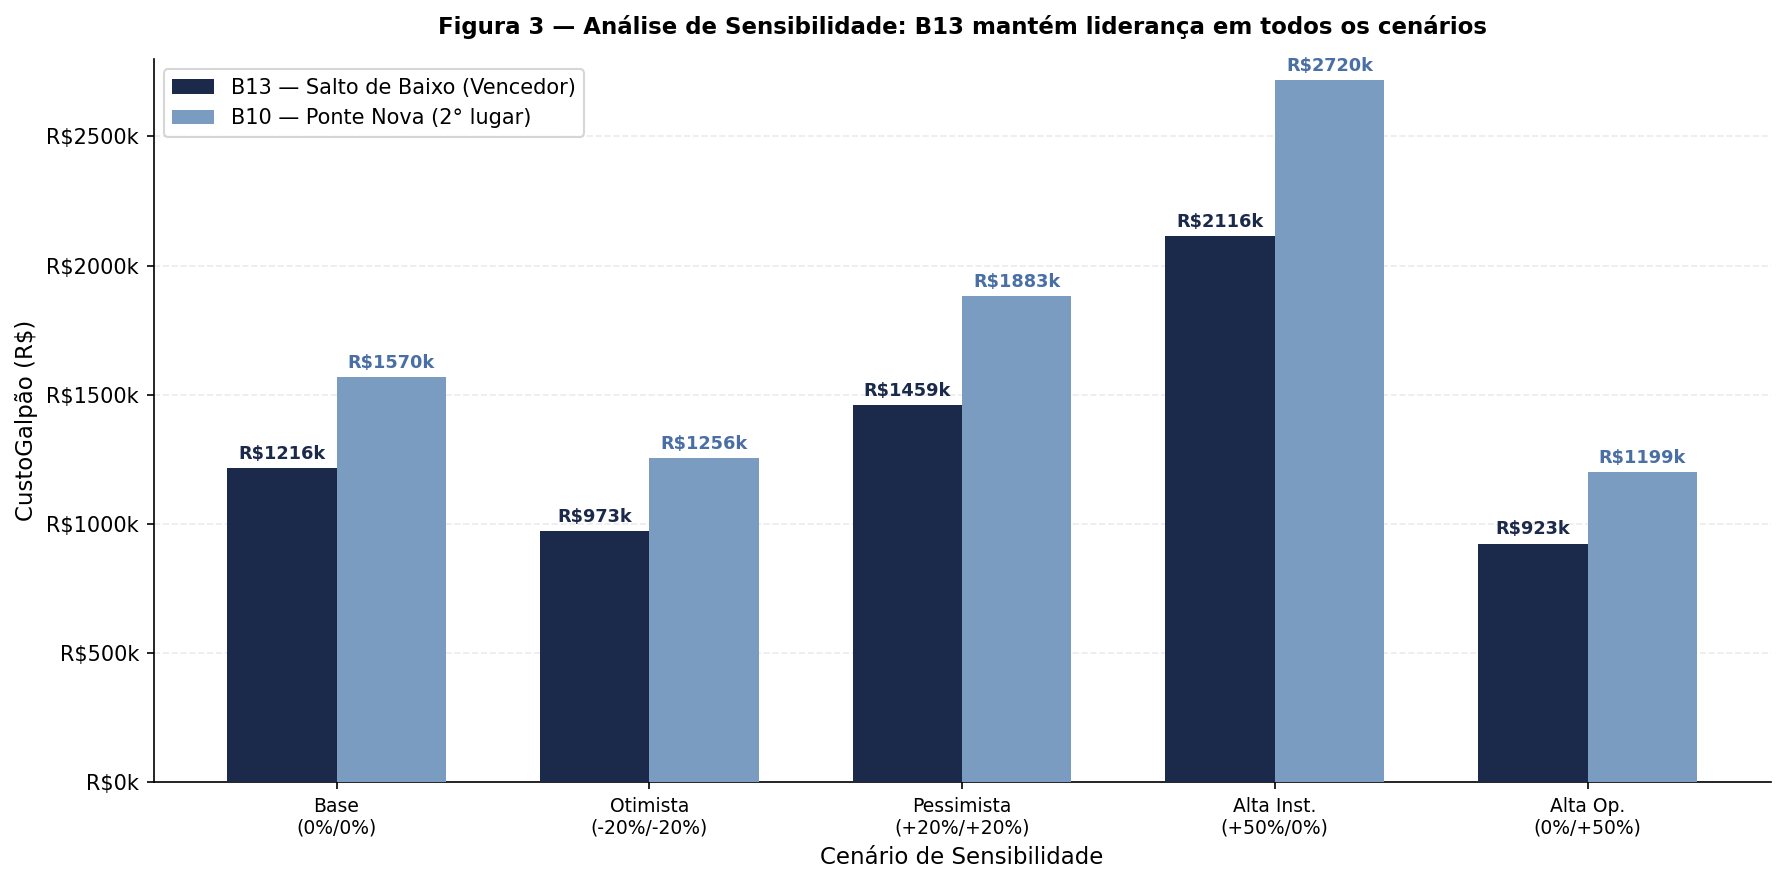
\includegraphics[width=0.95\textwidth]{figura3_sensibilidade.png}
\caption{Análise de sensibilidade: Bairro 13 mantém liderança em todos os cenários}
\label{fig:sensibilidade}
\end{figure}

O Bairro 13 -- Salto de Baixo manteve-se como o melhor candidato em todos os cinco cenários avaliados, demonstrando que a decisão é \textbf{robusta} a variações de até 50\% nos custos de instalação e operação. Este resultado fortalece a confiabilidade do modelo como ferramenta de apoio à decisão logística.

\subsection*{7.2 Validação com Dados Reais de Mercado}
Para validar o modelo proposto, compararam-se os resultados com as decisões reais de localização tomadas por empresas instaladas em Extrema-MG, com base em dados públicos de mercado.

As empresas instaladas em Extrema concentram-se principalmente em três regiões: (i) \textit{Bairro dos Pires (BR-381) -- Bairro 3}, onde se localizam a Fulwood S.A. (presente desde 2013, com Mercado Livre, Frigelar e Tok Stok como inquilinas) \cite{tudoep2023}, o BTLG Extrema e o Parque Logístico Extrema com 147.196 m² de ABL; (ii) \textit{Condomínio Logístico -- Bairro 6}, onde se localiza o VBI Log Extrema, único condomínio com acesso direto pela BR-381, com 121.611 m² de ABL e 100\% de ocupação \cite{vbi2024}; e (iii) \textit{Divisa SP/MG -- Bairro 7}, a apenas 2 km da divisa com São Paulo. Praticamente tudo que se constrói de galpões logísticos em Extrema é absorvido imediatamente \cite{galpaoaluguel2022}.

A comparação entre o resultado do modelo (Bairro 13 -- Salto de Baixo) e as decisões reais de mercado (Bairros 3, 6 e 14, próximos à BR-381) revela uma divergência esperada e academicamente relevante. O modelo otimiza exclusivamente a expressão \textit{custoGalpão = custoInstalação -- custoOperaçãoAnual}, priorizando bairros com menor custo fixo. As empresas reais consideram fatores adicionais não contemplados no modelo: (i) proximidade e acesso direto à BR-381; (ii) infraestrutura de condomínio classe A, com portaria 24h e docas; (iii) incentivos fiscais municipais e estaduais; e (iv) facilidade de acesso para veículos de grande porte.

Esta análise demonstra que o sistema proposto constitui uma ferramenta eficaz de apoio à decisão sob a perspectiva do custo financeiro modelado. A incorporação de restrições adicionais -- como proximidade de rodovias, infraestrutura e incentivos fiscais -- em versões futuras aproximaria os resultados computacionais das decisões reais de mercado, fortalecendo a aplicabilidade prática do sistema.

% ============================================================
% 8. CONCLUSAO
% ============================================================
\section*{8. CONCLUSÃO}

Este trabalho apresentou um sistema computacional para apoio à decisão logística baseado em grafos não direcionados, implementado com Orientação a Objetos em C++. O TAD \textit{Grafo} com lista de adjacência mostrou-se adequado para a modelagem de 15 bairros reais de Extrema-MG.

A comparação entre \textit{Dijkstra}, \textit{Bellman-Ford} e \textit{Floyd-Warshall} confirmou resultados idênticos para pesos positivos. O \textit{Dijkstra} foi o mais eficiente ($O(n^2)$), enquanto o \textit{Floyd-Warshall} ($O(n^3)$) e \textit{Bellman-Ford} ($O(n \times a)$) apresentaram tempos similares para o grafo de 15 vértices e 22 arestas.

O Bairro 13 -- Salto de Baixo -- foi indicado como o local mais adequado para instalação do galpão logístico em Extrema-MG, com o menor \textit{custoGalp\~ao} de R\$ 1.215.634,50. A escolha de Extrema mostrou-se plenamente justificada pela experiência profissional da autora e pelo reconhecimento acadêmico da cidade como polo logístico nacional \cite{cushman2022, gala2023, venceslau2024, ecommerce2023}.

Como limitações, as distâncias são estimativas via \textit{Google Maps} e as demandas mensais são estimativas, visto que dados reais são de natureza proprietária. Como trabalhos futuros, sugere-se a extensão do modelo para instâncias maiores, a incorporação de dados reais de demanda e a otimização dos algoritmos com filas de prioridade para reduzir a complexidade do \textit{dijkstra()} para $O((n+a)\log n)$.

% ============================================================
% REFERENCIAS
% ============================================================
\section*{REFERÊNCIAS}

\begin{thebibliography}{14}

\bibitem{ballou2006}
BALLOU, R. H. \textit{Gerenciamento da Cadeia de Suprimentos/Logística Empresarial}. 5. ed. Porto Alegre: Bookman, 2006.

\bibitem{bellman1958}
BELLMAN, R. On a routing problem. \textit{Quarterly of Applied Mathematics}, v. 16, n. 1, p. 87--90, 1958.

\bibitem{cormen2009}
CORMEN, T. H. et al. \textit{Introduction to Algorithms}. 3. ed. Cambridge: MIT Press, 2009.

\bibitem{cushman2022}
CUSHMAN \& WAKEFIELD. Polos Logísticos Brasileiros. \textit{Relatório de Análise Setorial}. São Paulo, 2022.

\bibitem{dasgupta2006}
DASGUPTA, S.; PAPADIMITRIOU, C.; VAZIRANI, U. \textit{Algorithms}. New York: McGraw-Hill, 2006.

\bibitem{dijkstra1959}
DIJKSTRA, E. W. A note on two problems in connexion with graphs. \textit{Numerische Mathematik}, v. 1, n. 1, p. 269--271, 1959.

\bibitem{gala2023}
GALA, P. A história do polo industrial de Extrema. \textit{Economia \& Finanças}, set. 2023.

\bibitem{neves2026a}
NEVES, T. \textit{Estruturas de Dados e Algoritmos: Análise de Algoritmos}. Notas de Aula. UFF, 2026.

\bibitem{neves2026b}
NEVES, T. \textit{Programação Estruturada em C++: Classes e Objetos}. Capítulo 8. UFF, 2026.

\bibitem{ecommerce2023}
REDAÇÃO E-COMMERCE BRASIL. Extrema, MG: o paradoxo logístico do Brasil. \textit{E-Commerce Brasil}, 2023.

\bibitem{sedgewick2011}
SEDGEWICK, R.; WAYNE, K. \textit{Algorithms}. 4. ed. Boston: Addison-Wesley Professional, 2011.

\bibitem{szwarcfiter2010}
SZWARCFITER, J. L.; MARKENZON, L. \textit{Estruturas de Dados e seus Algoritmos}. 3. ed. Rio de Janeiro: LTC, 2010.

\bibitem{venceslau2024}
VENCESLAU, I.; LIMA, F. L. S. Guerra dos lugares .com: a localização estratégica de Extrema (MG) para a logística do comércio eletrônico. \textit{Caminhos de Geografia}, v. 25, n. 102, p. 104--119, dez. 2024. DOI: 10.14393/RCG2510273062.

\bibitem{ziviani2011}
ZIVIANI, N. \textit{Projeto de Algoritmos com Implementações em Pascal e C}. 3. ed. São Paulo: Cengage Learning, 2011.

\bibitem{vbi2024}
VBI LOG EXTREMA. Condomínio Logístico VBI Log Extrema. Disponível em: vbiextrema.com.br. Acesso em: maio 2026.

\bibitem{tudoep2023}
TUDO EP. Extrema vai ganhar novo condomínio logístico com 75 mil m². \textit{Tudo EP}, jan. 2023. Disponível em: tudoep.com. Acesso em: maio 2026.

\bibitem{galpaoaluguel2022}
GALPÃO ALUGUEL E VENDA. Galpões logísticos em Extrema são disputados por empresas. Disponível em: galpaoaluguelevenda.com.br. Acesso em: maio 2026.

\end{thebibliography}

\vspace{1cm}
\begin{center}
\rule{\linewidth}{0.4pt} \\
\vspace{0.2cm}
{\small Claudineia Moreira de Oliveira -- PPGCM/UFF -- Junho de 2026}
\end{center}

\end{document}
